

\section{Doimiy magnit. Magnit maydon. Toklarning magnit maydoni.}


\begin{enumerate}

\item Quyida keltirilgan doimiy magnitlar haqidagi fikrlarning qaysi bir(lar)i to‘g‘ri yoki noto‘g‘ri ekanini aniqlang.
1) bir xil nomli qutblari o‘zaro tortishadi;
2) magnitlarni ikkiga bo‘lish orqali faqatgina bitta qutbli magnitni hosil qilish mumkin.
\begin{enumerate}[label=\Alph*)]
\item 1 – to‘g‘ri, 2 – to‘g‘ri.
\item 1 – to‘g‘ri, 2 – noto‘g‘ri.
\item 1 – noto‘g‘ri, 2 – noto‘g‘ri.
\item 1 – noto‘g‘ri, 2 – to‘g‘ri.
\end{enumerate}


\item Yerning qaysi nuqtalarida magnit mili aniq gorizontal holatda bo‘ladi?
\begin{enumerate}[label=\Alph*)]
\item shimoliy magnit qutbida.
\item janubiy magnit qutbida.
\item magnit ekvatorida.
\item geografik ekvatorda.
\end{enumerate}

\item O‘zgarmas tok o‘tayotgan o‘tkazgich atrofida qanday maydon bo‘ladi?
\begin{enumerate}[label=\Alph*)]
\item elektrostatik maydon.
\item hech qanday maydon bo‘lmaydi.
\item elektr va magnit maydon.
\item magnit maydon.
\end{enumerate}

\item To‘g‘ri chiziqli tokli o‘tkazgich magnit maydonining A nuqtasida maydon induksiya chizig‘ining yo‘nalishini toping. (Rasmga qarang)

\begin{tikzpicture}[>=stealth, scale=1.2]
  % Vertikal o'tkazgich
  \draw[thick] (0,2.5) -- (0,-1);
  \draw[->, thick] (0,0.5) -- (0,-0.5) node[right] {$I$};
  
  % Magnit maydon chizig'i (ellips)
  \draw[dashed] (0,1) ellipse (1.5 and 0.5);
  \draw[->] (-1.5,1) -- (-1.49,1.01); % Yo'nalish ko'rsatkichi
  
  % A nuqtasi
  \filldraw (1.3,0.8) circle (1pt) node[below right] {A};
  
  % Yo'nalish vektorlari (1, 2, 3, 4)
  \draw[->] (1.3,0.8) -- (1.3,0.2) node[below] {1}; % To'g'ri javob yo'nalishi
  \draw[->] (1.3,0.8) -- (2,0.8) node[right] {2};
  \draw[->] (1.3,0.8) -- (1.8,1.3) node[above right] {3};
  \draw[->] (1.3,0.8) -- (0.5,0.8) node[left] {4};
\end{tikzpicture}

\begin{enumerate}[label=\Alph*)]
\item 1.
\item 2.
\item 3.
\item 4.
\end{enumerate}


\item Quyidagi $I$ tokli o‘tkazgichning A nuqtadagi magnit maydon induksiya vektori rasmda ko‘rsatilgan qaysi yo‘nalish bilan mos tushadi? (Tok o‘tkazgichdan chizmaga kirmoqda)

\begin{tikzpicture}[>=stealth, scale=1.2]
  % A nuqtasi va koordinata o'qlari
  \filldraw (0,1.5) circle (1.5pt) node[above right] {A};
  \draw[->] (0,1.5) -- (-0.8,1.5) node[left] {1};
  \draw[->] (0,1.5) -- (0,2.3) node[above] {2};
  \draw[->] (0,1.5) -- (0.8,1.5) node[right] {3};
  \draw[->] (0,1.5) -- (0,0.7) node[below] {4};
  
  % Tok belgisi (chizmaga kiruvchi)
  \draw (0,0) circle (0.2);
  \draw (0.14,0.14) -- (-0.14,-0.14);
  \draw (-0.14,0.14) -- (0.14,-0.14);
  \node at (0.4,0) {$I$};
\end{tikzpicture}

\begin{enumerate}[label=\Alph*)]
\item 3.
\item 1.
\item 4.
\item 2.
\end{enumerate}

\item Quyidagi $I$ tokli o‘tkazgichning A nuqtadagi magnit maydon induksiya vektori rasmda ko‘rsatilgan qaysi yo‘nalish bilan mos tushadi? (Tok o‘tkazgichdan biz tomonga chiqmoqda)

\begin{tikzpicture}[>=stealth, scale=1.2]
  % A nuqtasi va koordinata o'qlari
  \filldraw (0,1.5) circle (1.5pt) node[above right] {A};
  \draw[->] (0,1.5) -- (0,2.3) node[above] {1};
  \draw[->] (0,1.5) -- (0.8,1.5) node[right] {2};
  \draw[->] (0,1.5) -- (0,0.7) node[below] {3};
  \draw[->] (0,1.5) -- (-0.8,1.5) node[left] {4};
  
  % Tok belgisi (biz tomonga chiquvchi)
  \draw (0,0) circle (0.2);
  \filldraw (0,0) circle (1.5pt);
  \node at (0.4,0) {$I$};
\end{tikzpicture}

\begin{enumerate}[label=\Alph*)]
\item 3.
\item 1.
\item 4.
\item 2.
\end{enumerate}

\item Quyidagi tokli o‘tkazgichning A nuqtadagi magnit maydon induksiya vektori rasmda ko‘rsatilgan qaysi yo‘nalish bilan mos tushadi?

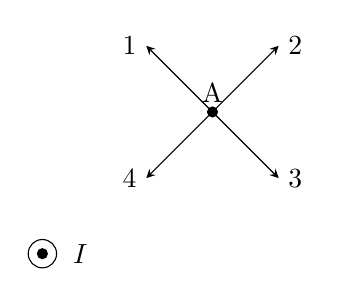
\begin{tikzpicture}[>=stealth, scale=1.2]
  % A nuqtasi
  \filldraw (0,1.5) circle (1.5pt) node[above] {A};
  
  % Yo'nalish vektorlari (X shaklida)
  \draw[->] (0,1.5) -- (-0.7,2.2) node[left] {1};  % Yuqori-chap
  \draw[->] (0,1.5) -- (0.7,2.2) node[right] {2};  % Yuqori-o'ng
  \draw[->] (0,1.5) -- (0.7,0.8) node[right] {3};  % Pastki-o'ng
  \draw[->] (0,1.5) -- (-0.7,0.8) node[left] {4};  % Pastki-chap
  
  % Tok belgisi (biz tomonga chiquvchi)
  \draw (-1.8,0) circle (0.15);
  \filldraw (-1.8,0) circle (1.5pt);
  \node at (-1.4,0) {$I$};
\end{tikzpicture}

\begin{enumerate}[label=\Alph*)]
\item 4.
\item 1.
\item 2.
\item 3.
\end{enumerate}

\item Muhitdagi cheksiz to‘g‘ri $I$ tokning o‘zidan $r$ masofada hosil qiladigan magnit maydon induksiyasining ifodasini ko‘rsating.
\begin{enumerate}[label=\Alph*)]
\item $\frac{\mu\mu_0 I}{2\pi r}$
\item $\frac{\mu\mu_0 I}{4\pi r}$
\item $\frac{\mu\mu_0 U}{4\pi r}$
\item $\frac{2\mu\mu_0 I}{\pi r}$
\end{enumerate}


\item Magnit maydon ikkita parallel va teng toklar tomonidan hosil qilingan (rasmga q.). A nuqtada magnit induksiya vektori qanday yo‘nalgan?

\begin{tikzpicture}[>=stealth, scale=1.5]
  % Gorizontal punktir chiziq
  \draw[dashed] (-2,0) -- (2,0);
  
  % Chapdagi tok (bizga chiquvchi - nuqta)
  \draw[thick] (-1.5,0) circle (0.15);
  \filldraw (-1.5,0) circle (1.5pt);
  \node at (-1.5,0.4) {$I$};
  
  % O'ngdagi tok (ichkariga kiruvchi - krest)
  \draw[thick] (1.5,0) circle (0.15);
  \draw (1.39,0.11) -- (1.61,-0.11);
  \draw (1.39,-0.11) -- (1.61,0.11);
  \node at (1.5,0.4) {$I$};
  
  % Vertikal punktir chiziq va A nuqtasi
  \draw[dashed] (0,0.5) -- (0,-0.8);
  \filldraw (0,-0.6) circle (1.5pt) node[right] {A};
\end{tikzpicture}

\begin{enumerate}[label=\Alph*)]
\item bizga.
\item pastga.
\item yuqoriga.
\item bizdan.
\end{enumerate}

\item Ikkita bir xil kuchli, o‘zaro parallel va ''bizdan`` yo‘nalgan to‘g‘ri chiziqli toklarning hosil qilgan magnit maydon induksiyasi A nuqtada qanday yo‘nalgan?

\begin{tikzpicture}[>=stealth, scale=1.5]
  % Gorizontal punktir chiziq
  \draw[dashed] (-2,0) -- (2,0);
  
  % Chapdagi tok (ichkariga kiruvchi - krest)
  \draw[thick] (-1.5,0) circle (0.15);
  \draw (-1.61,0.11) -- (-1.39,-0.11);
  \draw (-1.61,-0.11) -- (-1.39,0.11);
  \node at (-1.5,0.4) {$I$};
  
  % O'ngdagi tok (ichkariga kiruvchi - krest)
  \draw[thick] (1.5,0) circle (0.15);
  \draw (1.39,0.11) -- (1.61,-0.11);
  \draw (1.39,-0.11) -- (1.61,0.11);
  \node at (1.5,0.4) {$I$};
  
  % Vertikal punktir chiziq va A nuqtasi
  \draw[dashed] (0,0.5) -- (0,-0.8);
  \filldraw (0,-0.6) circle (1.5pt) node[right] {A};
\end{tikzpicture}

\begin{enumerate}[label=\Alph*)]
\item yuqoriga.
\item chapga.
\item nolga teng.
\item pastga.
\end{enumerate}

\item Ikkita bir xil kuchli, o‘zaro parallel va ''bizga`` yo‘nalgan to‘g‘ri chiziqli toklarning hosil qilgan magnit maydon induksiyasi A nuqtada qanday yo‘nalgan?

\begin{tikzpicture}[>=stealth, scale=1.5]
  % Gorizontal punktir chiziq
  \draw[dashed] (-2,0) -- (2,0);
  
  % Chapdagi tok (biz tomonga chiquvchi - nuqta)
  \draw[thick] (-1.5,0) circle (0.15);
  \filldraw (-1.5,0) circle (1.5pt);
  \node at (-1.5,0.4) {$I$};
  
  % O'ngdagi tok (biz tomonga chiquvchi - nuqta)
  \draw[thick] (1.5,0) circle (0.15);
  \filldraw (1.5,0) circle (1.5pt);
  \node at (1.5,0.4) {$I$};
  
  % Vertikal punktir chiziq va A nuqtasi
  \draw[dashed] (0,0.5) -- (0,-0.8);
  \filldraw (0,-0.6) circle (1.5pt) node[right] {A};
\end{tikzpicture}

\begin{enumerate}[label=\Alph*)]
\item o‘ngga.
\item yuqoriga.
\item nolga teng.
\item chapga.
\end{enumerate}

\item Bir-biridan $d$ masofada joylashgan va har biridan bir xil yo‘nalishda $I$ tok o‘tayotgan ikki o‘zaro parallel to‘g‘ri o‘tkazgichlarning o‘rtasidagi nuqtada magnit maydon induksiyasi qanday bo‘ladi?



\begin{enumerate}[label=\Alph*)]
\item $\mu_0 \frac{2I}{\pi d}$
\item $\mu_0 \frac{I}{\pi d}$
\item 0.
\item $\mu_0 \frac{I}{2\pi d}$
\end{enumerate}


\item Rasmda 4 juft tok unsurlari keltirilgan. Qaysi holda ular o‘zaro itarishadi?
\begin{enumerate}[label=\Alph*)]
\item $\uparrow \uparrow$.
\item $\uparrow \rightarrow$.
\item $\rightarrow \leftarrow$.
\item $\downarrow \uparrow$.
\end{enumerate}

\item Ma’lumki, ikkita proton bir-biridan Kulon kuchi vositasida itarishishadi. Qanday holatda ular bir-biriga tortiladi?
\begin{enumerate}[label=\Alph*)]
\item o‘zaro teskari parallel yo‘nalishda o‘ta katta tezlikda harakatlanganda.
\item o‘zaro bir xil yo‘nalishda parallel o‘ta katta tezlikda harakatlanganda.
\item o‘zaro teskari yo‘nalishda bir-biridan uzoqlashsa.
\item hech qachon ular tortishmaydilar.
\end{enumerate}

\item $I_1=10$ A tok o‘tayotgan birinchi o‘tkazgich o‘zidan 10 cm uzoqlikda unga parallel joylashgan ikkinchi o‘tkazgichning har 1 m uzunligini $4 \cdot 10^{-4}$ N kuch bilan itarayotgan bo‘lsa, ikkinchi o‘tkazgichdan o‘tayotgan tok necha Amper va qaysi yo‘nalishda oqmoqda?

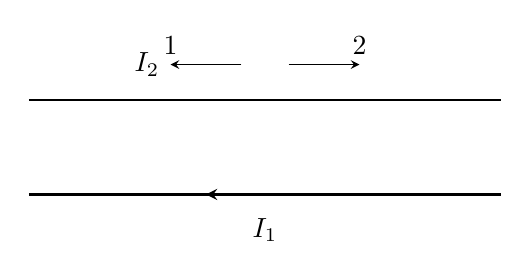
\begin{tikzpicture}[>=stealth, scale=1.5]
  % Pastki o'tkazgich (I1)
  \draw[thick] (-2,0) -- (2,0);
  \draw[->, thick] (0.5,0) -- (-0.5,0);
  \node at (0,-0.3) {$I_1$};
  
  % Yuqorigi o'tkazgich (I2)
  \draw[thick] (-2,0.8) -- (2,0.8);
  \node at (-1,1.1) {$I_2$};
  
  % Yo'nalish ko'rsatkichlari (1 va 2)
  \draw[->] (-0.2,1.1) -- (-0.8,1.1) node[above] {1};
  \draw[->] (0.2,1.1) -- (0.8,1.1) node[above] {2};
\end{tikzpicture}

\begin{enumerate}[label=\Alph*)]
\item 10 A; 1-yo‘nalishda.
\item 20 A; 2-yo‘nalishda.
\item 15 A; 1-yo‘nalishda.
\item 15 A; 2-yo‘nalishda.
\end{enumerate}

\item Keltirilgan ta’riflardan qaysi birida tok kuchi birligi (1 A) to‘g‘ri aniqlangan?
\begin{enumerate}[label=\Alph*)]
\item induktivligi 1 H bo‘lgan g‘altak hosil qilayotgan oqim 1 Wb bo‘lgandagi tok.
\item o‘tkazgich kesimidan 1 s da 1 C zaryad o‘tgandagi tok.
\item qarshiligi 1 $\Omega$ bo‘lgan o‘tkazgichdan o‘tgan tok.
\item vakuumda 1 m masofada parallel o‘tkazgichlar orasidagi $2 \cdot 10^{-7}$ N kuchni vujudga keltiruvchi tok.
\end{enumerate}

\end{enumerate}



\begin{table}[!ht]
\centering
\begin{tabular}{|c|c|c|c|c|c|c|c|}
\hline
1c & 2c & 3d & 4a & 5a & 6b & 7b & 8a \\ \hline
9c & 10b & 11a & 12c & 13d & 14b & 15b & 16d \\ \hline
\end{tabular}
\end{table}









\section{Amper kuchi}



\begin{enumerate}

\item Magnit maydonning tokli o‘tkazgichga ta’sir kuchi (Amper kuchi) ni ifodalaydigan formulani ko‘rsating.
\begin{enumerate}[label=\Alph*)]
\item $F = IBL\cos\alpha$.
\item $F = kq_1q_2/r^2$.
\item $F = Eq$.
\item $F = IBL\sin\alpha$.
\end{enumerate}

\item Induksiyasi 20 T bo‘lgan bir jinsli magnit maydonda 3 A tok o‘tayotgan o‘tkazgich rasmdagidek joylashgan. Unga ta’sir qilayotgan Amper kuchining modulini toping (N). O‘tkazgichning aktiv qismining uzunligi 40 cm. $\alpha=37^\circ$.

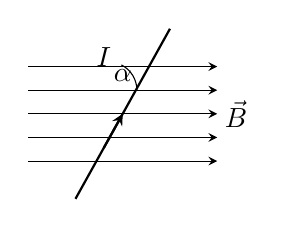
\begin{tikzpicture}[>=stealth, scale=1.2]
  % Magnit maydon induksiya chiziqlari (B)
  \foreach \y in {0, 0.25, 0.5, 0.75, 1.0} {
    \draw[->, thin] (-1, \y) -- (1, \y);
  }
  \node at (1.2, 0.5) {$\vec{B}$};
  
  % Tokli o'tkazgich
  \draw[thick] (-0.5, -0.4) -- (0.5, 1.4);
  \draw[->, thick] (-0.2, 0.14) -- (0, 0.5); % Tok yo'nalishi ko'rsatkichi
  \node at (-0.2, 1.1) {$I$};
  
  % Alfa burchagi
  \draw (0.15, 0.75) arc (0:63:0.3);
  \node at (0, 0.9) {$\alpha$};
\end{tikzpicture}

\begin{enumerate}[label=\Alph*)]
\item 14,4.
\item 12,8.
\item 10,2.
\item 16,4.
\end{enumerate}

\item Induksiyasi 2 T bo‘lgan bir jinsli magnit maydonga kiritilgan 8 cm uzunlikdagi o‘tkazgichdan 4 A tok oqayotgan bo‘lsa, bu o‘tkazgichga maydon tomonidan qanday kuch ta’sir qiladi (N)? Tok va magnit induksiya vektori orasidagi burchak $30^\circ$ ga teng.
\begin{enumerate}[label=\Alph*)]
\item 0,4.
\item 0,24.
\item 0,32.
\item 1,25.
\end{enumerate}

\item Aktiv qismining uzunligi 0,4 m bo‘lgan o‘tkazgich induksiyasi 0,8 T bo‘lgan bir jinsli magnit maydoniga kiritilganda unga 1,6 N kuch ta’sir etdi. O‘tkazgich magnit induksiya chiziqlariga perpendikulyar joylashgan bo‘lsa, undagi tok kuchini aniqlang (A).
\begin{enumerate}[label=\Alph*)]
\item 5.
\item 4.
\item 3.
\item 2.
\end{enumerate}

\item Induksiyasi 40 mT bo‘lgan magnit maydon aktiv qismining uzunligi 10 cm bo‘lgan to‘g‘ri o‘tkazgichga 60 mN kuch bilan ta’sir etmoqda. O‘tkazgichdagi tok kuchi 30 A. O‘tkazgich magnit maydon induksiyasi vektori bilan qanday burchak hosil qiladi?
\begin{enumerate}[label=\Alph*)]
\item $90^\circ$.
\item $60^\circ$.
\item $45^\circ$.
\item $30^\circ$.
\end{enumerate}

\setcounter{enumi}{5}
\item Induksiyasi 2 T bo‘lgan bir jinsli magnit maydonda uzunligi 0,2 m bo‘lgan o‘tkazgich joylashgan. Agar o‘tkazgichdan o‘tayotgan o‘zgarmas tok kuchi 5 A bo‘lsa, magnit maydon tomonidan o‘tkazgichga ta’sir etuvchi maksimal va minimal kuchlar nimaga teng bo‘lishi mumkin (N)?
\begin{enumerate}[label=\Alph*)]
\item 2; 0.
\item 2; 1.
\item 10; 2.
\item 1; 0.
\end{enumerate}

\item Vakuumda magnit kuchlanganligi $H=5000$ A/m bo‘lgan magnit maydon hosil qilindi. U yerga uzunligi 20 cm bo‘lgan va 10 A tok o‘tayotgan o‘tkazgich joylashtirildi. Tok va magnit induksiyasi yo‘nalishlari o‘zaro $53^\circ$ burchak hosil qilsa, Amper kuchi qanday (mN) bo‘ladi? $\sin 53^\circ = 0,8$, $\pi=3$.
\begin{enumerate}[label=\Alph*)]
\item 9,6.
\item 2.
\item 2,3.
\item 4,5.
\end{enumerate}

\item Induksiyasi 5 T bo‘lgan magnit maydonda uzunligi 20 cm bo‘lgan o‘tkazgich bo‘lib, undan 10 A tok o‘tmoqda. Agar o‘tkazgich magnit induksiyasi yo‘nalishi bilan $30^\circ$ burchak hosil qilsa, unga maydon tomonidan necha Nyuton kuch ta’sir qiladi?
\begin{enumerate}[label=\Alph*)]
\item 10.
\item 1,5.
\item 5.
\item 18.
\end{enumerate}

\item Magnit induksiya chiziqlariga tik joylashgan tokli o‘tkazgichga 2,8 N kuch ta’sir etmoqda. O‘tkazgich bilan induksiya chiziqlari orasidagi burchak $30^\circ$ bo‘lganda, ta’sir kuchi qanday bo‘ladi (N)?
\begin{enumerate}[label=\Alph*)]
\item 0,7.
\item 1,4.
\item 1,96.
\item 2,4.
\end{enumerate}

\item Bir jinsli magnit maydon induksiyasi vektori va tokli to‘g‘ri o‘tkazgich orasidagi $30^\circ$ burchak 2 marta orttirilsa, o‘tkazgichga ta’sir qiluvchi Amper kuchi qanday o‘zgaradi?
\begin{enumerate}[label=\Alph*)]
\item 2 marta ortadi.
\item 2 marta kamayadi.
\item $\sqrt{2}$ marta ortadi.
\item $\sqrt{3}$ marta ortadi.
\end{enumerate}

\setcounter{enumi}{10}
\item Aktiv qismining uzunligi 10 cm bo‘lgan o‘tkazgichdagi tok kuchi 2 A ga teng. U magnit induksiyasi 0,08 T bo‘lgan bir jinsli magnit maydonda turibdi. O‘tkazgich induksiya chiziqlariga perpendikulyar ravishda 10 cm siljiganda necha mJ ish bajariladi?
\begin{enumerate}[label=\Alph*)]
\item 32.
\item 0,8.
\item 3,2.
\item 1,6.
\end{enumerate}

\item Induksiyasi 20 mT bo‘lgan bir jinsli magnit maydon chiziqlariga tik joylashgan 8 cm uzunlikdagi simdan 50 A tok oqmoqda. Bu sim o‘ziga tik yo‘nalishda induksiya chiziqlariga $45^\circ$ burchak ostida ko‘chganida tok 8 mJ ish bajargan bo‘lsa, sim qanday (cm) masofaga ko‘chgan?
\begin{enumerate}[label=\Alph*)]
\item 10,2.
\item 13,2.
\item 14,1.
\item 15,2.
\end{enumerate}

\item Uzunligi 0,1 m bo‘lgan 5 A tokli o‘tkazgichni bir jinsli magnit maydonda induksiya chiziqlariga va o‘ziga tik yo‘nalishda 20 mm masofaga siljitishda 0,01 J ish bajariladi. Magnit maydon induksiyasi necha Tesla?
\begin{enumerate}[label=\Alph*)]
\item 0,1.
\item 1.
\item 2.
\item 0,2.
\end{enumerate}

\item Uzunligi 20 cm bo‘lgan 2 A tokli o‘tkazgich bir jinsli magnit maydon induksiya chiziqlariga perpendikulyar yo‘nalishda 10 cm siljiganda, 32 mJ ish bajarildi. Magnit maydon induksiyasini toping (T).
\begin{enumerate}[label=\Alph*)]
\item 0,04.
\item 0,08.
\item 0,4.
\item 0,8.
\end{enumerate}

\item Uzunligi 80 cm bo‘lgan o‘tkazgich induksiyasi 0,4 T bo‘lgan bir jinsli magnit maydonda 0,15 m/s tezlik bilan induksiya chiziqlariga va o‘ziga tik yo‘nalishda tekis harakat qilmoqda. Agar 10 s ichida 0,96 J ish bajarilgan bo‘lsa, o‘tkazgichdagi tok kuchi qanday (A) bo‘ladi?
\begin{enumerate}[label=\Alph*)]
\item 0,4.
\item 1.
\item 2.
\item 1,8.
\end{enumerate}

\item Yuzi $S=1,2$ m$^2$ bo‘lgan 2 A tokli ramka induksiyasi 30 T bo‘lgan bir jinsli magnit maydonda joylashgan. Ramka normali va induksiya chiziqlari orasidagi burchak $53^\circ$ ga teng. Ramkaga ta’sir qiluvchi kuch momenti nimaga teng (N$\cdot$m)?
\begin{enumerate}[label=\Alph*)]
\item 16,8.
\item 64,2.
\item 57,6.
\item 28,5.
\end{enumerate}

\end{enumerate}




\begin{table}[!ht]
\centering
\begin{tabular}{|c|c|c|c|c|c|c|c|}
\hline
1d & 2a & 3c & 4a & 5d & 6a & 7a & 8c \\ \hline
9b & 10d & 11d & 12c & 13b & 14d & 15c & 16c \\ \hline
\end{tabular}
\end{table}












\section{Lorens kuchi}



\begin{enumerate}

\item Quyidagilar ichidan Lorens kuchining ifodasini toping.
\begin{enumerate}[label=\Alph*)]
\item $qvB\sin\alpha$.
\item $qvB\cos\alpha$.
\item $vB/2$.
\item $vB\sin\alpha$.
\end{enumerate}

\item Induksiyasi 20 T bo‘lgan magnit maydonga 0,2 C zaryadga ega zarra 25 m/s tezlik bilan induksiya chiziqlariga $53^\circ$ burchak ostida uchib kirdi. Unga ta’sir qilayotgan Lorens kuchini toping (N).
\begin{enumerate}[label=\Alph*)]
\item 100.
\item 20.
\item 30.
\item 80.
\end{enumerate}

\item Induksiyasi 4 T bo‘lgan bir jinsli magnit maydonga $10^7$ m/s tezlik bilan induksiya chiziqlariga perpendikulyar yo‘nalishda uchib kirgan elektronga ta’sir etuvchi kuchning moduli qanday (N)? $e = -1,6 \cdot 10^{-19}$ C.
\begin{enumerate}[label=\Alph*)]
\item $6,4 \cdot 10^{-12}$.
\item $0,4 \cdot 10^{-7}$.
\item $0,14 \cdot 10^{-12}$.
\item $3,2 \cdot 10^{-12}$.
\end{enumerate}

\item Induksiyasi 0,2 T bo‘lgan magnit maydonda induksiya chiziqlariga tik ravishda 10 Mm/s tezlik bilan harakatlanayotgan protonga qanday kuch ta’sir qiladi (pN). $e = 1,6 \cdot 10^{-19}$ C.
\begin{enumerate}[label=\Alph*)]
\item 0,5.
\item 0,16.
\item 0,32.
\item 0,64.
\end{enumerate}

\item Magnit kuch chiziqlariga tik yo‘nalishda 2 km/s tezlik bilan harakatlanayotgan 0,4 C zaryadga ta’sir qilayotgan Lorens kuchi 8 N ga teng bo‘lsa, magnit induksiyasi qanday?
\begin{enumerate}[label=\Alph*)]
\item 10 mT.
\item 10 T.
\item 1,6 mT.
\item 1,6 T.
\end{enumerate}

\item Induksiyasi 0,2 T bo‘lgan magnit maydonga induksiya chiziqlariga tik ravishda elektron uchib kirdi. Unga ta’sir etuvchi kuch $0,32 \cdot 10^{-12}$ N bo‘lsa, uning tezligi qanday (m/s)? $e = 1,6 \cdot 10^{-19}$ C.
\begin{enumerate}[label=\Alph*)]
\item $1,6 \cdot 10^5$.
\item $1 \cdot 10^7$.
\item $32 \cdot 10^5$.
\item $6,4 \cdot 10^4$.
\end{enumerate}

\item Protonning tezligi 24 marta kamayganda va magnit maydon induksiyasi 12 marta ortganda, magnit maydon tomonidan protonga ta’sir qiluvchi Lorens kuchi qanday o‘zgaradi?
\begin{enumerate}[label=\Alph*)]
\item 2 marta ortadi.
\item 4 marta kamayadi.
\item 4 marta ortadi.
\item 2 marta kamayadi.
\end{enumerate}


\item Magnit maydonda harakatlanayotgan manfiy zaryadlangan zarrachaga ta’sir etuvchi Lorens kuchi yo‘nalishi chizmada ko‘rsatilgan qaysi yo‘nalish bilan mos tushadi? Magnit maydon kuch chiziqlarari bizdan chizma tekisligiga tik yo‘nalgan.

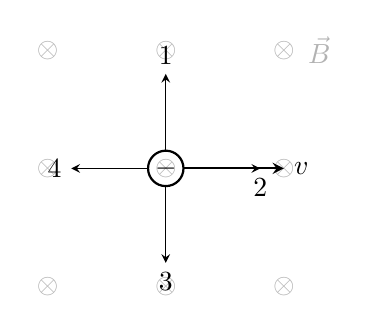
\begin{tikzpicture}[>=stealth, scale=1.5]
  % Magnit maydon induksiyasi (krestlar - bizdan ichkariga)
  \foreach \x in {-1, 0, 1} {
    \foreach \y in {-1, 0, 1} {
      \node[gray!60] at (\x, \y) {$\otimes$};
    }
  }
  \node[gray!60] at (1.3, 1) {$\vec{B}$};

  % Markaziy manfiy zaryad
  \draw[thick] (0,0) circle (0.15);
  \node at (0,0) {$-$};
  
  % Tezlik vektori (v)
  \draw[->, thick] (0.15,0) -- (1,0) node[right] {$v$};
  
  % Yo'nalish ko'rsatkichlari (1, 2, 3, 4)
  \draw[->] (0, 0.15) -- (0, 0.8) node[above] {1}; % Yuqoriga
  \draw[->] (0.5, 0) -- (0.8, 0) node[below] {2};  % O'ngga
  \draw[->] (0, -0.15) -- (0, -0.8) node[below] {3}; % Pastga
  \draw[->] (-0.15, 0) -- (-0.8, 0) node[left] {4}; % Chapga
\end{tikzpicture}

\begin{enumerate}[label=\Alph*)]
\item 1.
\item 3.
\item 4.
\item 2.
\end{enumerate}

\item Harakatlanayotgan musbat zaryadli zarraga magnit maydon tomonidan ta’sir etadigan Lorens kuchining yo‘nalishini aniqlang. Maydonning magnit induksiyasi vektori chizma tekisligiga tik va bizdan chizmaga tomon yo‘nalgan ($\otimes$).

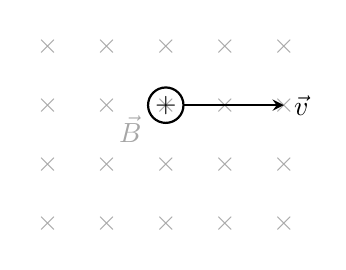
\begin{tikzpicture}[>=stealth, scale=1.5]
  % Magnit maydon induksiyasi (krestlar - bizdan ichkariga)
  \foreach \x in {-1, -0.5, 0, 0.5, 1} {
    \foreach \y in {-0.5, 0, 0.5, 1} {
      \node[gray!70] at (\x, \y) {$\times$};
    }
  }
  \node[gray!70] at (-0.3, 0.3) {$\vec{B}$};

  % Markaziy musbat zaryad
  \draw[thick] (0,0.5) circle (0.15);
  \node at (0,0.5) {$+$};
  
  % Tezlik vektori (v)
  \draw[->, thick] (0.15,0.5) -- (1,0.5) node[right] {$\vec{v}$};
  
 \end{tikzpicture}

\begin{enumerate}[label=\Alph*)]
\item o‘ngga.
\item pastga.
\item yuqoriga.
\item chapga.
\end{enumerate}

\item Elektron rasmda ko‘rsatilganidek, bir jinsli magnit maydoniga uchib kiradi. Unga magnit maydoni tomonidan ta’sir qiladigan kuch qaysi tomonga yo‘naladi?

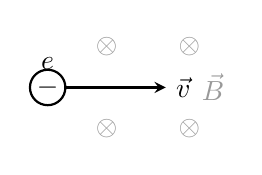
\begin{tikzpicture}[>=stealth, scale=1.5]
  % Magnit maydon induksiyasi (krestlar - bizdan ichkariga)
  \foreach \x in {0.5, 1.2} {
    \foreach \y in {0, 0.7} {
      \node[gray!80] at (\x, \y) {$\otimes$};
    }
  }
  \node[gray!80] at (1.4, 0.35) {$\vec{B}$};

  % Elektron (e)
  \draw[thick] (0,0.35) circle (0.15);
  \node at (0,0.55) {$e$};
  \node at (0,0.35) {$-$};
  
  % Tezlik vektori (v)
  \draw[->, thick] (0.15,0.35) -- (1,0.35) node[right] {$\vec{v}$};
  
  
\end{tikzpicture}

\begin{enumerate}[label=\Alph*)]
\item o‘ngga.
\item pastga.
\item yuqoriga.
\item chapga.
\end{enumerate}


\item Tezligi $v$ bo‘lgan $q$ zaryad induksiyasi $B$ bo‘lgan magnit maydonga kuch chiziqlariga tik ravishda uchib kirdi. Shu zaryad harakat traektoryasining egrilik radiusi qaysi ifoda asosida hisoblanishi mumkin?
\begin{enumerate}[label=\Alph*)]
\item $mv/qB$.
\item $qv/mB$.
\item $qB/mv$.
\item $vB/qm$.
\end{enumerate}

\item Tezligi $v$ va zaryadi $q$ bo‘lgan ion induksiyasi $B$ bo‘lgan bir jinsli magnit maydonga kiradi va $R$ radiusli aylana chizadi. Ionning massasi qanday ifoda vositasida hisoblanadi?
\begin{enumerate}[label=\Alph*)]
\item $qvB/R$.
\item $qvR/B$.
\item $qBR/v$.
\item $B/qvR$.
\end{enumerate}

\item Induksiyasi 20 T bo‘lgan magnit maydonga 0,08 g massali 0,002 C zaryadga ega zarra 25 m/s tezlik bilan induksiya chiziqlariga tik ravishda uchib kirdi. Uning aylanish radiusini (cm) va aylanish davrini (ms) toping.
\begin{enumerate}[label=\Alph*)]
\item 5; 4,76.
\item 8; 12,56.
\item 4; 4,76.
\item 5; 12,56.
\end{enumerate}

\item Induksiyasi 9,1 mT bo‘lgan bir jinsli magnit maydonga induksiya chiziqlariga perpendikulyar ravishda 16 Mm/s tezlik bilan uchib kirgan elektron harakat traektoryasining egrilik radiusini toping (cm). $m = 9,1 \cdot 10^{-31}$ kg, $e = 1,6 \cdot 10^{-19}$ C.
\begin{enumerate}[label=\Alph*)]
\item 100.
\item 10.
\item 0,1.
\item 1.
\end{enumerate}

\item Elektron induksiyasi 5 mT bo‘lgan magnit maydonga uchib kirib, 4 cm radiusli aylana bo‘ylab harakatlana boshlasa, uning tezligi qanday (m/s)?
\begin{enumerate}[label=\Alph*)]
\item $6 \cdot 10^6$.
\item 1000.
\item $3,5 \cdot 10^7$.
\item $5 \cdot 10^7$.
\end{enumerate}

\item Proton induksiyasi 20 mT bo‘lgan bir jinsli magnit maydonda 5 cm radiusli aylana chizdi. Proton zaryadi $1,6 \cdot 10^{-19}$ C bo‘lsa, uning impulsini aniqlang (kg$\cdot$m/s).
\begin{enumerate}[label=\Alph*)]
\item $3,2 \cdot 10^{-20}$.
\item $5 \cdot 10^{-21}$.
\item $1,6 \cdot 10^{-22}$.
\item $8 \cdot 10^{-22}$.
\end{enumerate}

\item Bir xil tezlikka ega bo‘lgan ikkita bir xil zaryadlangan zarralar magnit maydonga kuch chiziqlariga tik yo‘nalishda kirib, egrilik radiuslari $R_2 = 3R_1$ munosabatda bo‘lgan traektoriya bo‘yicha harakat qila boshladilar. 2-zarra massasi $m_2$ ning 1-zarra massasi $m_1$ ga nisbati $m_2/m_1$ qanday?
\begin{enumerate}[label=\Alph*)]
\item 0,5.
\item 1/3.
\item 2.
\item 3.
\end{enumerate}


\item Massasi $m$, zaryadi $q$ bo‘lgan zarracha induksiyasi $B$ bo‘lgan bir jinsli magnit maydonda aylana bo‘ylab harakatlanmoqda. Aylanish davrini toping.
\begin{enumerate}[label=\Alph*)]
\item $\pi m / 2qB$.
\item $\pi m / qB$.
\item $2\pi m / qB$.
\item $2\pi r^2 / v$.
\end{enumerate}

\item Agar bir jinsli magnit maydonda elektronning aylanish davri 9 ns bo‘lsa magnit maydon induksiyasi necha mT bo‘ladi? Elektronning zaryadi $1,6 \cdot 10^{-19}$ C, massasi $9,1 \cdot 10^{-31}$ kg.
\begin{enumerate}[label=\Alph*)]
\item 4,5.
\item 8.
\item 9.
\item 4.
\end{enumerate}

\item Induksiyasi 16,7 mT bo‘lgan bir jinsli magnit maydonga induksiya chiziqlariga tik yo‘nalishda uchib kirgan proton aylana traektoriya bo‘ylab harakatlanadi. Protonning 3,14 s ichidagi aylanishlar sonini toping. $e = 1,6 \cdot 10^{-19}$ C, $m_p = 1,67 \cdot 10^{-27}$ kg.
\begin{enumerate}[label=\Alph*)]
\item $4 \cdot 10^5$.
\item $8 \cdot 10^5$.
\item $3 \cdot 10^6$.
\item $6 \cdot 10^6$.
\end{enumerate}

\item Magnit induksiyasi 16,7 mT bo‘lgan bir jinsli magnit maydoniga induksiya chiziqlariga tik yo‘nalishda uchib kirgan proton aylana traektoriya bo‘ylab harakatlanadi. $6\pi$ s ichida protonning aylanishlar soni qanchaga teng bo‘ladi?
\begin{enumerate}[label=\Alph*)]
\item $6,2 \cdot 10^5$.
\item $4 \cdot 10^5$.
\item $6,2 \cdot 10^6$.
\item $4,8 \cdot 10^6$.
\end{enumerate}

\end{enumerate}




\begin{table}[!ht]
\centering
\begin{tabular}{|c|c|c|c|c|c|c|c|c|c|c|}
\hline
1a & 2d & 3a & 4c & 5a & 6b & 7d & 8b & 9c & 10b & 11a \\ \hline
12c & 13d & 14d & 15c & 16c & 17d & 18c & 19d & 20b & 21d & \\ \hline
\end{tabular}
\end{table}












\section{Magnit oqimi}


\begin{enumerate}

\item O‘lchov birliklarining xalqaro sistemasida magnit oqimining birligi qanday?
\begin{enumerate}[label=\Alph*)]
\item Kulon.
\item Tesla.
\item Veber.
\item Amper.
\end{enumerate}

\item Radiusi $r=20$ cm bo‘lgan xalqa induksiyasi $B=0,3$ T bo‘lgan bir jinsli magnit maydonda joylashgan. Induksiya vektori xalqa normali bilan $\alpha=37^\circ$ burchak hosil qiladi. Xalqani kesib o‘tuvchi magnit oqimini toping (mWb). $\pi=3$.

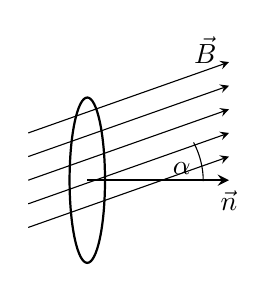
\begin{tikzpicture}[>=stealth, scale=1.5]
  % Xalqa (perspektivada ellips ko'rinishida)
  \draw[thick] (0,0) ellipse (0.15 and 0.7);
  
  % Magnit maydon chiziqlari (B) - tepaga va o'ngga yo'nalgan
  \foreach \i in {-2,-1,0,1,2} {
    \draw[->, thin] (-0.5, 0.2*\i) -- (1.2, 0.2*\i + 0.6);
  }
  \node at (1.0, 1.1) {$\vec{B}$};
  
  % Normal vektor (n) - sirtga tik, pastga va o'ngga yo'nalgan
  \draw[->, thick] (0,0) -- (1.2, 0) node[below] {$\vec{n}$};
  
  % Alfa burchagi (n va B chiziqlari orasida)
  \draw (0.9, 0.32) arc (28:0:0.7);
  \node at (0.8, 0.1) {$\alpha$};
\end{tikzpicture}

\begin{enumerate}[label=\Alph*)]
\item 3,14.
\item 10.
\item 28,8.
\item 15.
\end{enumerate}

\item Yuzi 0,2 m$^2$ bo‘lgan kontur induksiyasi 5 T bo‘lgan bir jinsli magnit maydonda joylashgan. Agar kontur tekisligi induksiya chiziqlariga parallel joylashgan bo‘lsa, kontur yuzidan o‘tayotgan magnit oqimi necha Veber bo‘ladi?
\begin{enumerate}[label=\Alph*)]
\item 0.
\item 0,1.
\item 0,5.
\item 1.
\end{enumerate}

\item To‘g‘ri to‘rtburchak shaklidagi ramkani induksiyasi 6,5 T bo‘lgan magnit maydon rasmdagi kabi kesib o‘tmoqda. Unga tushayotgan magnit oqimini toping (Wb).


\begin{tikzpicture}[>=stealth, x={(1.2cm,0cm)}, y={(0cm,1.2cm)}, z={(-0.6cm,-0.4cm)}, scale=1.8]
  % Koordinata o'qlari
  \draw[->] (0,0,0) -- (1.8,0,0) node[right] {x};
  \draw[->] (0,0,0) -- (0,1.3,0) node[above] {y};
  \draw[->] (0,0,0) -- (0,0,1.8) node[below left] {z};
  
  % To'g'ri to'rtburchakli ramka (yz-tekisligida)
  \draw[thick] (0,0,0) -- (0,1,0) -- (0,1,1.5) -- (0,0,1.5) -- cycle;
  
  % O'lchamlar va yozuvlar
  \node[left, rotate=90] at (0,1,0) {20 cm};
  \node[below, sloped] at (0,0,1.5) {40 cm};
  
  % Magnit induksiya vektori (B)
  \draw[->, very thick] (0,0.5,0.75) -- (1.5,0.5,0.75) node[right] {$\vec{B}$};
  
  % Perpendikulyarlik belgilari (B vektori y va z o'qlariga tikligini ko'rsatadi)
  \draw (0.15,0.5,0.75) -- (0.15,0.65,0.75) -- (0,0.65,0.75);
 
\end{tikzpicture}

\begin{enumerate}[label=\Alph*)]
\item 0,52.
\item 0,27.
\item 0,39.
\item 0,48.
\end{enumerate}

\item Radiusi 5 cm bo‘lgan doirasimon yuza induksiyasi 2 T bo‘lgan bir jinsli magnit maydonda joylashgan. Induksiya vektori doira sirti normali bilan $0^\circ$ burchak hosil qiladi. Sirtni kesib o‘tuvchi magnit oqimini toping (mWb).
\begin{enumerate}[label=\Alph*)]
\item 3,14.
\item 10.
\item 30,5.
\item 15,7.
\end{enumerate}

\item Tomonlari 4 cm dan bo‘lgan teng tomonli uchburchak induksiyasi 2 T bo‘lgan bir jinsli magnit maydonda joylashgan. Induksiya vektori uchburchak sirti normali bilan $30^\circ$ burchak hosil qiladi. Sirtni kesib o‘tuvchi magnit oqimini toping (mWb). 
\begin{enumerate}[label=\Alph*)]
\item $0,8\sqrt{3}$.
\item $0,4\sqrt{3}$.
\item $0,4\sqrt{6}$.
\item 1,2.
\end{enumerate}

\item Yuzi 2 m$^2$ bo‘lgan va magnit maydon induksiyasi vektoriga tik joylashgan yassi konturdan 10 Wb magnit oqim o‘tsa, magnit induksiyasi qanday (T)?
\begin{enumerate}[label=\Alph*)]
\item 0,2.
\item 0,4.
\item 2,5.
\item 5.
\end{enumerate}

\item Magnit maydon induksiyasi vektoriga tik bo‘lgan yassi konturdan 6 Wb magnit oqim o‘tadi. Agar magnit induksiyasi 3 T bo‘lsa, konturning yuzi qanday (m$^2$)?
\begin{enumerate}[label=\Alph*)]
\item 0,5.
\item 2/3.
\item 2.
\item 12.
\end{enumerate}

\item Magnit induksiyasi 4 T bo‘lgan maydonda joylashgan 1 cm radiusli xalqani kesib o‘tayotgan magnit oqim 0,628 mWb bo‘lishi uchun magnit induksiya vektori bilan halqa tekisligi orasidagi burchak qanday bo‘lishi kerak?
\begin{enumerate}[label=\Alph*)]
\item $0^\circ$.
\item $30^\circ$.
\item $45^\circ$.
\item $60^\circ$.
\end{enumerate}

\item Magnit maydon oqimi ortadi, agar ...
1) magnit maydon induksiyasi ortsa;
2) magnit maydon induksiyasi kamaysa;
3) magnit maydon kesib o‘tuvchi yuza kamaysa;
4) magnit maydon kesib o‘tuvchi yuza ortsa.
\begin{enumerate}[label=\Alph*)]
\item 2, 3.
\item 1, 3.
\item 1, 4.
\item 2, 4.
\end{enumerate}

\item Quyidagi hollarning qaysi birida ramka yuzasidan o‘tuvchi magnit induksiya oqimi o‘zgarmaydi? 
\begin{enumerate}[label=\Alph*)]
\item bir jinsli magnit maydonda o‘z tekisligidan o‘tuvchi o‘q atrofida aylanganida.
\item bir jinsli bo‘lmagan magnit maydonda ilgarilanma harakat qilganida.
\item bir jinsli bo‘lmagan magnit maydonda aylanganida.
\item bir jinsli magnit maydonda ilgarilanma harakat qilganida.
\end{enumerate}

\item Yuzi 25 cm$^2$ bo‘lgan sim ramka bir jinsli magnit maydonda aylantirilganda, ramkani kesib o‘tuvchi magnit oqim $\Phi=2,5 \cdot 10^{-4}\cos 6t$ (Wb) qonun bo‘yicha o‘zgaradi. Magnit maydon induksiyasi qanday (T)? 
\begin{enumerate}[label=\Alph*)]
\item 0,1.
\item 0,6.
\item 1.
\item 0,2.
\end{enumerate}

\item Magnit maydonda harakatlanayotgan 5 A tokli kontur bilan chegaralangan yuzadan o‘tuvchi magnit oqim 0,4 mWb dan 0,8 mWb ga o‘zgargan bo‘lsa, necha milliJoul ish bajarilgan?
\begin{enumerate}[label=\Alph*)]
\item 2.
\item 3.
\item 1.
\item 4.
\end{enumerate}

\item Induksiyasi $4/\pi$ T bo‘lgan bir jinsli magnit maydonda diametri 10 cm bo‘lgan va 1 A tok o‘tayotgan o‘ram bor. O‘ramning tekisligi magnit induksiya vektoriga parallel. O‘ramni uning tekisligi magnit induksiya vektoriga tik bo‘ladigan qilib $90^\circ$ ga burish uchun necha Joul ish bajarish kerak? 
\begin{enumerate}[label=\Alph*)]
\item $10^{-2}$.
\item $\pi \cdot 10^{-4}$.
\item $10^{-4}$.
\item $\pi \cdot 10^{-2}$.
\end{enumerate}

\end{enumerate}



\begin{table}[!ht]
\centering
\begin{tabular}{|c|c|c|c|c|c|c|c|c|c|c|}
\hline
1c & 2c & 3a & 4a & 5d & 6d & 7d & 8c & 9b & 10c & 11d \\ \hline
12a & 13a & 14a & & & & & & & & \\ \hline
\end{tabular}
\end{table}


